\documentclass{article}

\usepackage{graphicx}
\usepackage{hyperref}
\usepackage{tikz}
\usepackage{pgfplots}
\usepackage{placeins}

\author{Eugen Croitoru}
\title{Minimal \LaTeX example}

\begin{document}
\maketitle

\section{Introduction}
\subsection{Motivation}

\section{Method}
We'll probably use Rastrigin's Function\cite{Rastrigin}:

$$ f(x) = A \cdot n + \sum_{i=1}^n \left[ x_i^2 - A \cdot cos(2 \pi x_i) \right],
A = 10, x_i \in \left[ -5.12, 5.15 \right]$$



\section{Experiments}

Some of the experiments we have tried as part of the optimization problem.

\begin{enumerate} 
	\item Genetic algorithm
	\begin{enumerate}
		\item \label{experiment:1a} Low crossover probability: 
		\begin{itemize}
			\item crossover probability: 0.1
			\item bit mutation probability: 0.01
			\item chromosome mutation probability: 0.1
			\item selection: roulette
		\end{itemize} 
		\item \label{experiment:1b} High crossover probability:
		\begin{itemize}
			\item crossover probability: 0.6
			\item bit mutation probability: 0.01
			\item chromosome mutation probability: 0.1
			\item selection: roulette
		\end{itemize}
	\end{enumerate} 

	\item Hill Climbing
	\begin{enumerate}
		\item \label{experiment:2a} best selection
		\item \label{experiment:2b} first selection
	\end{enumerate}

	\item Hybrid Hill Climbing
	\begin{enumerate}
		\item \label{experiment:3a} \ref{experiment:1a} with \ref{experiment:2a}
	\end{enumerate}
  
\end{enumerate}

\section{Results}

\subsection{Griewangk}

\begin{figure}[!htbp]
\begin{tabular}{||c|||l|l|l||}
  \hline
  Experiment & Min & Max & Mean \\ \hline \hline
  \ref{experiment:1a} & 11.26 & 28.92 & 17.30 \\ \hline
  \ref{experiment:1b} & 12.33 & 29.62 & 19.89 \\ \hline
  \ref{experiment:2a} & 2.56-09 & 2.56-09 & 2.56-09 \\ \hline
  \ref{experiment:2b} & 0.03 & 2.56-09 & 0.40 \\ \hline
  \ref{experiment:3a} & 0.001 & 2.56-09 & 0.04 \\ \hline
\end{tabular}
\caption{minimum, maximum and the mean values for each experiment}
\end{figure}
\FloatBarrier

\subsubsection{Genetic Algorithm}
\begin{figure}[!htbp]
	\centering
	\begin{minipage}{.48\textwidth}
		\centering
		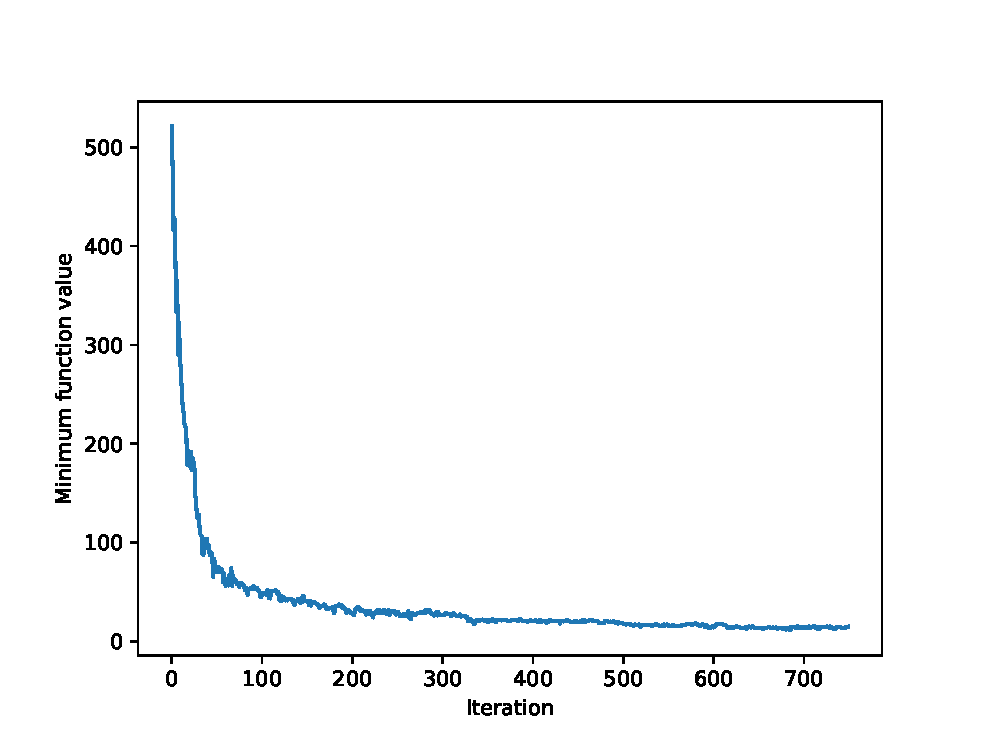
\includegraphics[scale=.4]{experiment_1a_griewangk/min_eval_0.eps}
		\caption{Function value}
	\end{minipage}\hfill
	\begin{minipage}{.48\textwidth}
		\centering
		\includegraphics[scale=.4]{experiment_1a_griewangk/max_fitness_0.eps}
		\caption{Fitness value}
	\end{minipage}
\end{figure}
\FloatBarrier

\begin{figure}[!htbp]
	\centering
	\begin{minipage}{.48\textwidth}
		\centering
		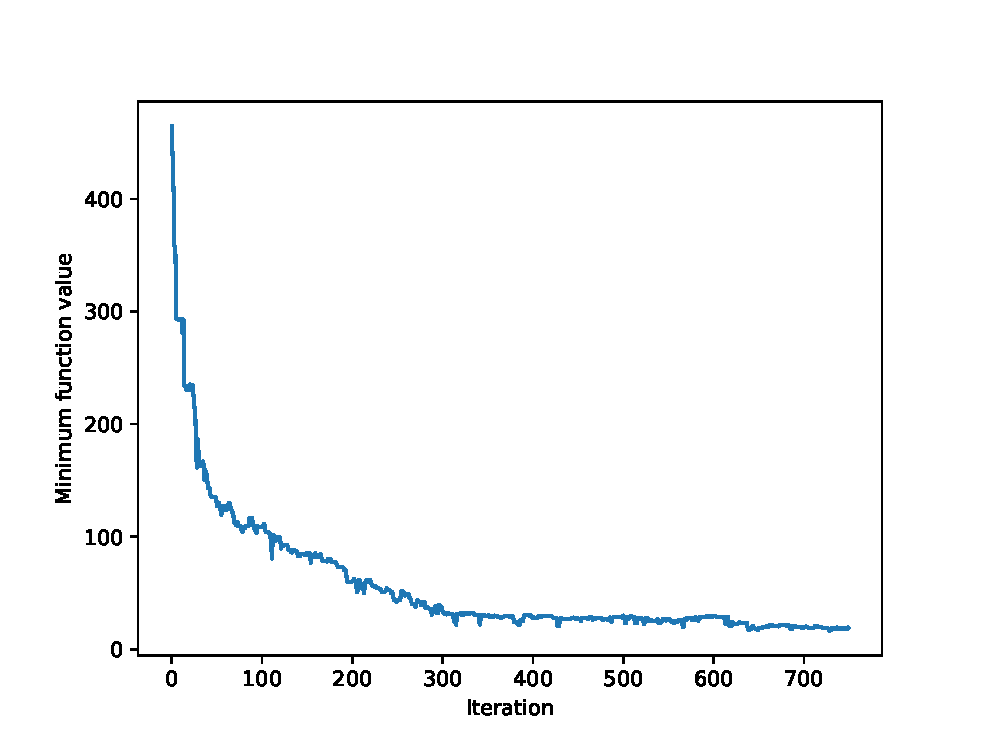
\includegraphics[scale=.4]{experiment_1b_griewangk/min_eval_0.eps}
		\caption{Function value}
	\end{minipage}\hfill
	\begin{minipage}{.48\textwidth}
		\centering
		\includegraphics[scale=.4]{experiment_1b_griewangk/max_fitness_0.eps}
		\caption{Fitness value}
	\end{minipage}
\end{figure}
\FloatBarrier

\subsubsection{Hill Climbing}
\begin{figure}[!htbp]
	\centering
	\begin{minipage}{.48\textwidth}
		\centering
		\includegraphics[scale=.4]{experiment_2a_griewangk/max_fitness_0.eps}
		\caption{Best improvement}
	\end{minipage}\hfill
	\begin{minipage}{.48\textwidth}
		\centering
		\includegraphics[scale=.4]{experiment_2b_griewangk/max_fitness_0.eps}
		\caption{First improvement}
	\end{minipage}\hfill
\end{figure}
\FloatBarrier

\subsubsection{Hybrid}
\begin{figure}[!htbp]
	\centering
	\begin{minipage}{.48\textwidth}
		\centering
		\includegraphics[scale=.4]{experiment_3a_griewangk/ga_min_eval_0.eps}
		\caption{Genetic algorithm}
	\end{minipage}\hfill
	\begin{minipage}{.48\textwidth}
		\centering
		\includegraphics[scale=.4]{experiment_3a_griewangk/hc_max_fitness_0.eps}
		\caption{Hill Climbing}
	\end{minipage}\hfill
\end{figure}
\FloatBarrier

\subsubsection{Interpretation}
\begin{figure}[!htbp]
	\centering
	\begin{minipage}{\textwidth}
		\centering
		\includegraphics[scale=.8]{boxplots/griewangk_boxplot.eps}
		\caption{Griewangk experiments boxplot}
		\label{fig:griewangk_experiments_boxplot}
	\end{minipage}\hfill
\end{figure}
\FloatBarrier

\begin{figure}[!htbp]
	\centering
	\begin{minipage}{\textwidth}
		\centering
		\includegraphics[scale=.8]{t_test/griewangk_t_test_matrix.png}
		\caption{Griewangk experiments t test matrix}
		\label{fig:griewangk_experiments_t_test}
	\end{minipage}\hfill
\end{figure}
\FloatBarrier
\paragraph{Observations} We can observe in Fig. \ref{fig:griewangk_experiments_boxplot} that the experiments \ref{experiment:1a} and \ref{experiment:1b} have the worst results but we can't really say which of the other three is the best. The t test does not give a significant p value to affirm that the experiments means differ.

\subsection{Rastrigin}

\begin{figure}[!htbp]
	\begin{tabular}{||c|||l|l|l||}
		\hline
		Experiment & Min & Max & Mean \\ \hline \hline
		\ref{experiment:1a} & 44.09 & 85.05 & 64.57  \\ \hline
		\ref{experiment:1b} & 50.77 & 107.90 & 76.33 \\ \hline
		\ref{experiment:2a} & 26.78 & 59.28 & 44.77  \\ \hline
		\ref{experiment:2b} & 50.97 & 76.22 & 57.91  \\ \hline
		\ref{experiment:3a} & 24.30 & 39.43 & 32.16  \\ \hline
	\end{tabular}
	\caption{minimum, maximum and the mean values for each experiment}
\end{figure}
\FloatBarrier

\subsubsection{Genetic Algorithm}
\begin{figure}[!htbp]
	\centering
	\begin{minipage}{.48\textwidth}
		\centering
		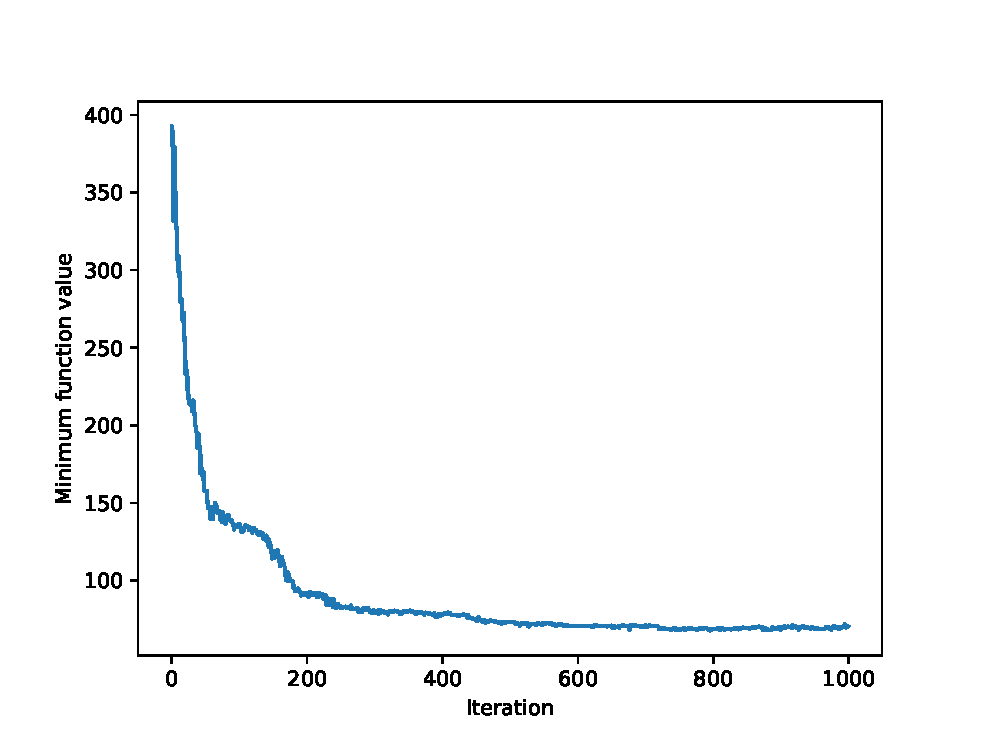
\includegraphics[scale=.4]{experiment_1a_rastrigin/min_eval_0.eps}
		\caption{Function value}
	\end{minipage}\hfill
	\begin{minipage}{.48\textwidth}
		\centering
		\includegraphics[scale=.4]{experiment_1a_rastrigin/max_fitness_0.eps}
		\caption{Fitness value}
	\end{minipage}
\end{figure}
\FloatBarrier

\begin{figure}[!htbp]
	\centering
	\begin{minipage}{.48\textwidth}
		\centering
		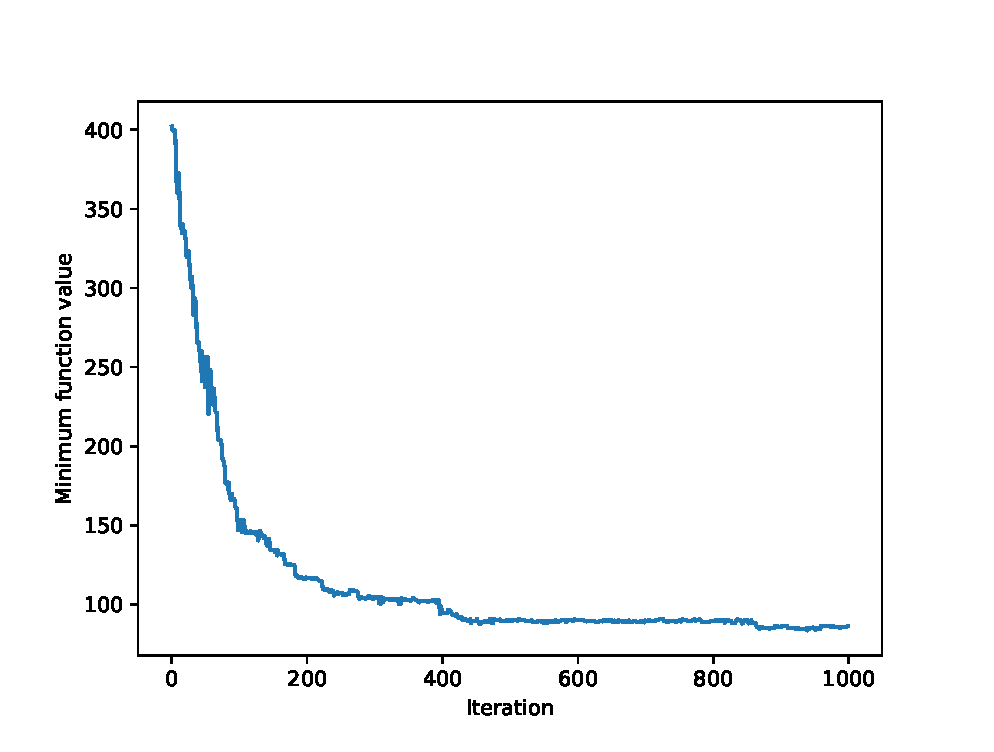
\includegraphics[scale=.4]{experiment_1b_rastrigin/min_eval_0.eps}
		\caption{Function value}
	\end{minipage}\hfill
	\begin{minipage}{.48\textwidth}
		\centering
		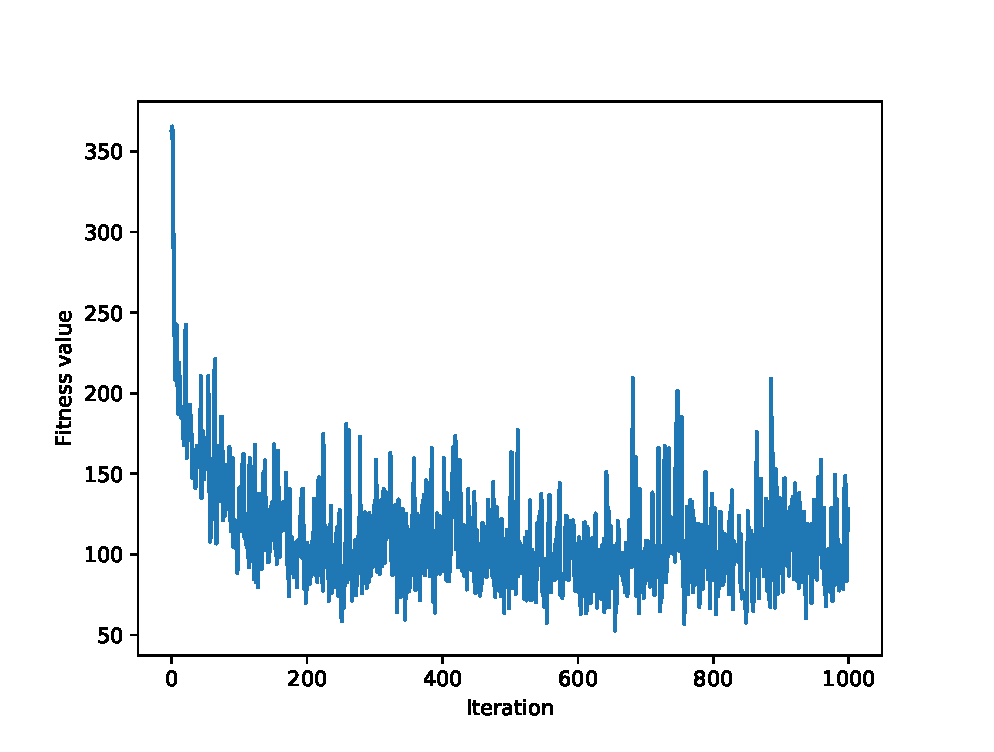
\includegraphics[scale=.4]{experiment_1b_rastrigin/max_fitness_0.eps}
		\caption{Fitness value}
	\end{minipage}
\end{figure}
\FloatBarrier
\subsubsection{Hill Climbing}
\begin{figure}[!htbp]
	\centering
	\begin{minipage}{.48\textwidth}
		\centering
		\includegraphics[scale=.4]{experiment_2a_rastrigin/max_fitness_0.eps}
		\caption{Best improvement}
	\end{minipage}\hfill
	\begin{minipage}{.48\textwidth}
		\centering
		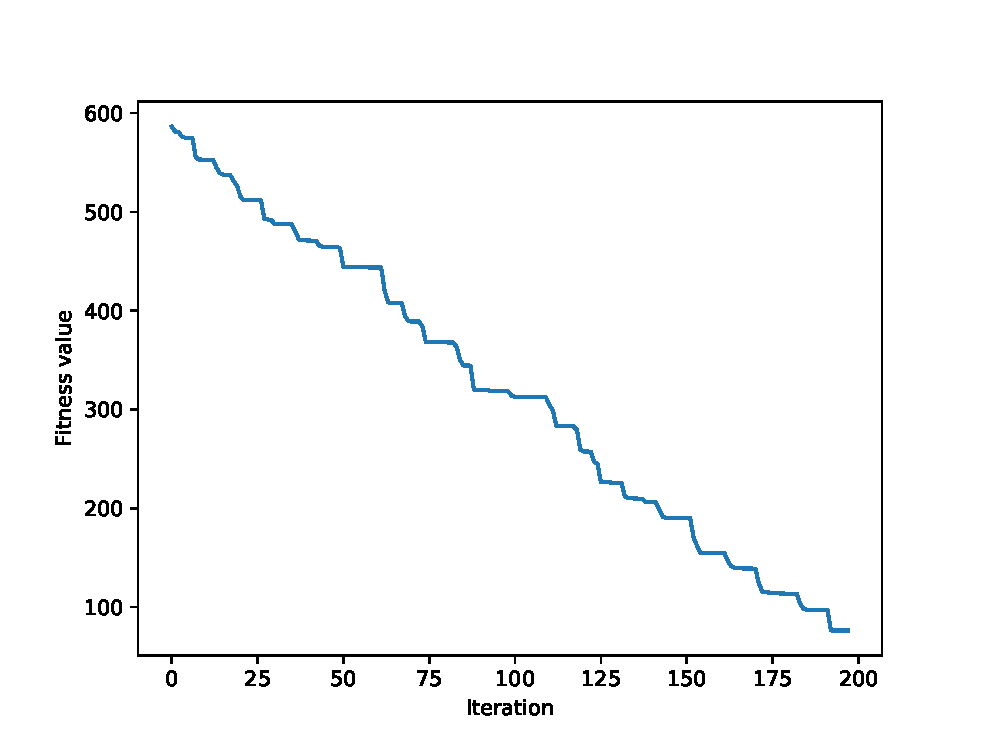
\includegraphics[scale=.4]{experiment_2b_rastrigin/max_fitness_0.eps}
		\caption{First improvement}
	\end{minipage}\hfill
\end{figure}
\FloatBarrier

\subsubsection{Hybrid}
\begin{figure}[!htbp]
	\centering
	\begin{minipage}{.48\textwidth}
		\centering
		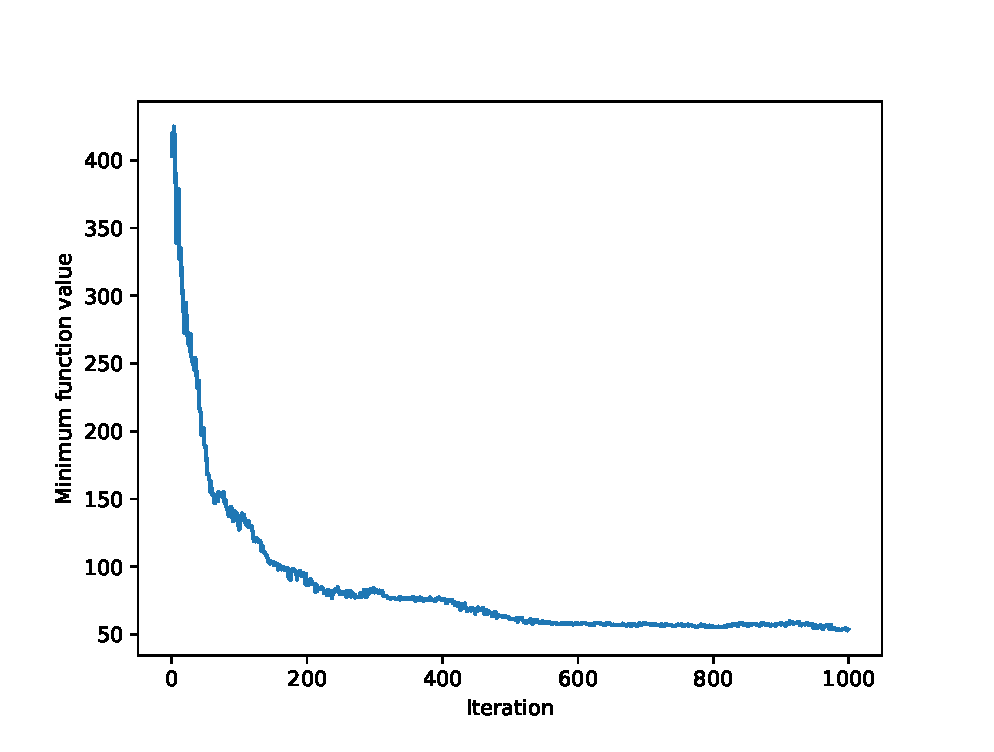
\includegraphics[scale=.4]{experiment_3a_rastrigin/ga_min_eval_0.eps}
		\caption{Genetic algorithm}
	\end{minipage}\hfill
	\begin{minipage}{.48\textwidth}
		\centering
		\includegraphics[scale=.4]{experiment_3a_rastrigin/hc_max_fitness_0.eps}
		\caption{Hill Climbing}
	\end{minipage}\hfill
\end{figure}
\FloatBarrier

\subsubsection{Interpretation}
\begin{figure}[!htbp]
	\centering
	\begin{minipage}{\textwidth}
		\centering
		\includegraphics[scale=.8]{boxplots/rastrigin_boxplot.eps}
		\caption{Rastrigin experiments boxplot}
		\label{fig:rastrigin_experiments_boxplot}
	\end{minipage}\hfill
\end{figure}
\FloatBarrier

\begin{figure}[!htbp]
	\centering
	\begin{minipage}{\textwidth}
		\centering
		\includegraphics[scale=.8]{t_test/rastrigin_t_test_matrix.png}
		\caption{Rastrigin experiments t test matrix}
		\label{fig:rastrigin_experiments_t_test}
	\end{minipage}\hfill
\end{figure}
\FloatBarrier

\paragraph{Observations} We can observe in Fig. \ref{fig:rastrigin_experiments_boxplot} that the experiment \ref{experiment:3a} goes to the best minimum value. This conclusion is also verified using t test. We can see that in Fig. \ref{fig:rastrigin_experiments_t_test} which shows the p value between experiments.

\subsection{Rosenbrock}

\begin{figure}[!htbp]
	\begin{tabular}{||c|||l|l|l||}
		\hline
		Experiment & Min & Max & Mean \\ \hline \hline
		\ref{experiment:1a} & 154.07 & 398.18 & 253.27 \\ \hline
		\ref{experiment:1b} & 109.52 & 382.73 & 272.65 \\ \hline
		\ref{experiment:2a} & 28.13 & 122.93 & 37.68   \\ \hline
		\ref{experiment:2b} & 25.25 & 132.46 & 33.21   \\ \hline
		\ref{experiment:3a} & 23.09 & 136.88 & 26.88  \\ \hline
	\end{tabular}
	\caption{minimum, maximum and the mean values for each experiment}
\end{figure}
\FloatBarrier

\subsubsection{Genetic Algorithm}
\begin{figure}[!htbp]
	\centering
	\begin{minipage}{.48\textwidth}
		\centering
		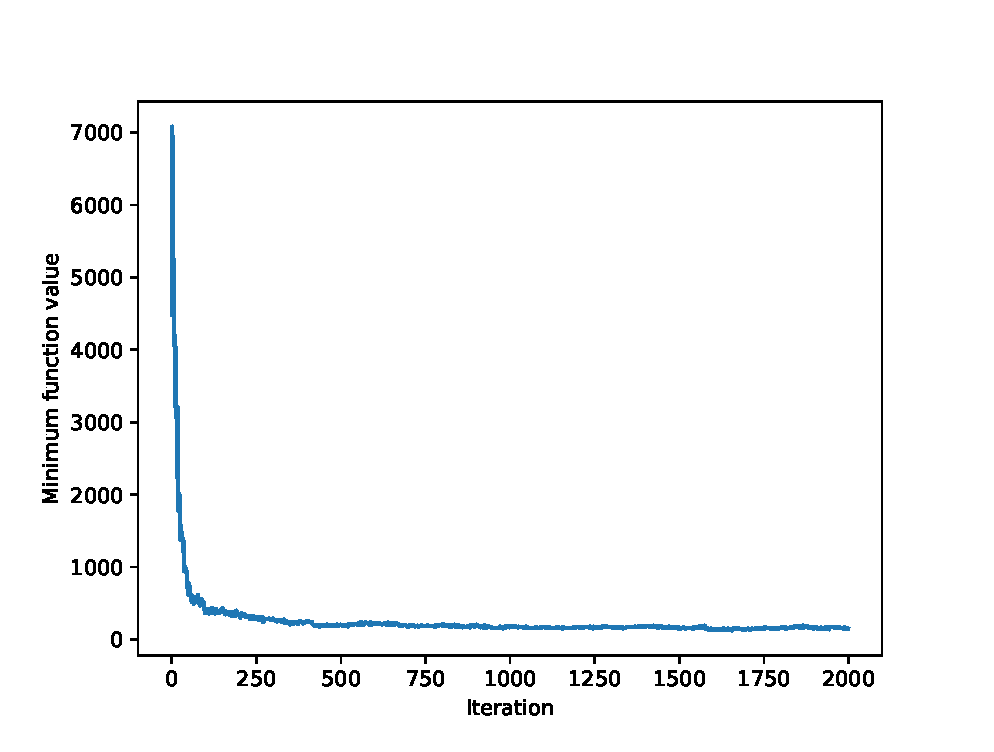
\includegraphics[scale=.4]{experiment_1a_rosenbrock/min_eval_0.eps}
		\caption{Function value}
	\end{minipage}\hfill
	\begin{minipage}{.48\textwidth}
		\centering
		\includegraphics[scale=.4]{experiment_1a_rosenbrock/max_fitness_0.eps}
		\caption{Fitness value}
	\end{minipage}
\end{figure}
\FloatBarrier

\begin{figure}[!htbp]
	\centering
	\begin{minipage}{.48\textwidth}
		\centering
		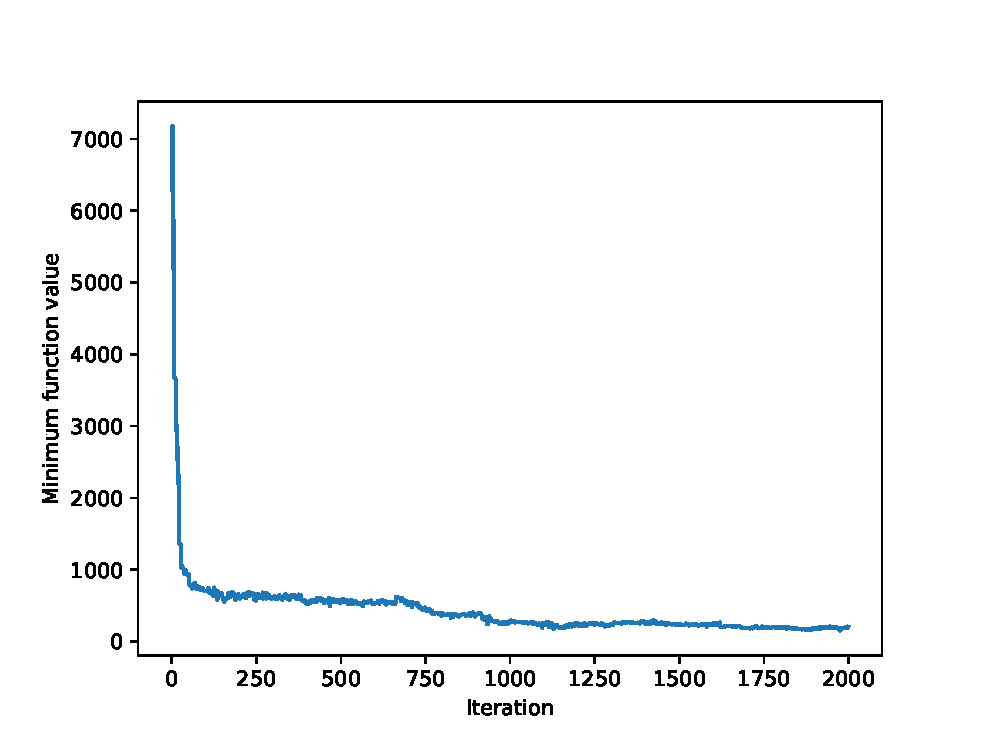
\includegraphics[scale=.4]{experiment_1b_rosenbrock/min_eval_0.eps}
		\caption{Function value}
	\end{minipage}\hfill
	\begin{minipage}{.48\textwidth}
		\centering
		\includegraphics[scale=.4]{experiment_1b_rosenbrock/max_fitness_0.eps}
		\caption{Fitness value}
	\end{minipage}
\end{figure}
\FloatBarrier

\subsubsection{Hill Climbing}
\begin{figure}[!htbp]
	\centering
	\begin{minipage}{.48\textwidth}
		\centering
		\includegraphics[scale=.4]{experiment_2a_rosenbrock/max_fitness_0.eps}
		\caption{Best improvement}
	\end{minipage}\hfill
	\begin{minipage}{.48\textwidth}
		\centering
		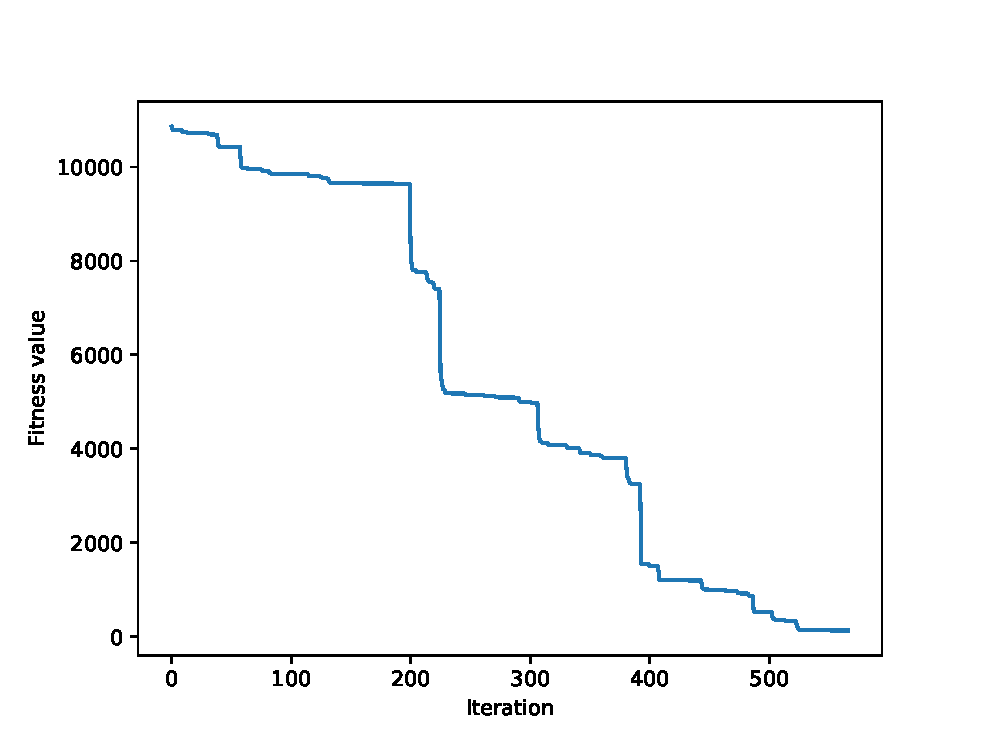
\includegraphics[scale=.4]{experiment_2b_rosenbrock/max_fitness_0.eps}
		\caption{First improvement}
	\end{minipage}\hfill
\end{figure}
\FloatBarrier

\subsubsection{Hybrid}
\begin{figure}[!htbp]
	\centering
	\begin{minipage}{.48\textwidth}
		\centering
		\includegraphics[scale=.4]{experiment_3a_rosenbrock/ga_min_eval_0.eps}
		\caption{Genetic algorithm}
	\end{minipage}\hfill
	\begin{minipage}{.48\textwidth}
		\centering
		\includegraphics[scale=.4]{experiment_3a_rosenbrock/hc_max_fitness_0.eps}
		\caption{Hill Climbing}
	\end{minipage}\hfill
\end{figure}
\FloatBarrier

\subsubsection{Interpretation}
\begin{figure}[!htbp]
	\centering
	\begin{minipage}{\textwidth}
		\centering
		\includegraphics[scale=.8]{boxplots/rosenbrock_boxplot.eps}
		\caption{Rosenbrock experiments boxplot}
	\end{minipage}\hfill
\end{figure}
\FloatBarrier

\begin{figure}[!htbp]
	\centering
	\begin{minipage}{\textwidth}
		\centering
		\includegraphics[scale=.8]{t_test/rosenbrock_t_test_matrix.png}
		\caption{Rosenbrock experiments t test matrix}
	\end{minipage}\hfill
\end{figure}
\FloatBarrier

\paragraph{Observations} //TODO:

\section{Conclusions}



\begin{thebibliography}{9}

\bibitem{wikipedia}
  Wikipedia Commons \\ Rastrigin's Function rendered image.
  \url{https://commons.wikimedia.org/wiki/Main_Page}

\bibitem{Rastrigin}
  Rastrigin, L. A. "Systems of extremal control." Mir, Moscow (1974).
\end{thebibliography}  
\end{document}
